% 第 8 章 一阶项与全阶展开
% 来源：docs/paper-submission/main.tex §"The first-order term: a parabolic series"
%       （Lemma model、Lemma finite、Lemma derbounds、Prop diff、Theorem D、Prop higher、Theorem E、
%       Remarks、Numerics）；一般化改写见 sec-general.tex（Theorem gen-D）与
%       docs/general-statements-zh.md §2.6；思路见 docs/mrr-first-order-zh.md。
% 数值：mrr_derivative.py、mrr_second.py（论文 Numerics）；kappa_variation.py（docs/kappa-variation-zh.md §3）；
%       图 figures/fig8_deficit.py（调用 docs/generality_check.py）。
\providecommand{\cfR}{\mathcal R}
\providecommand{\cfS}{\mathcal S}
\providecommand{\cfG}{\mathcal G}
\providecommand{\cfA}{\mathcal A}     % 吸引 Abel 时间（轨道级数）
\providecommand{\Arg}{\operatorname{Arg}}

\chapter{一阶项与全阶展开}\label{ch:first-order}

第~\ref{ch:confluence} 章证明了 $\tau_n(s)\to B_n\ee^{2\pi\ii na}$，但没有给出速率。
第~\ref{ch:confluence} 章末尾的数值表显示（数值），偏差与内蕴参数 $p=-\log\lambda_1\log\lambda_2$ 成正比：
\[
 \log\frac{\tau_n}{B_n\ee^{2\pi\ii na}}\approx\kappa^{(n)}p .
\]
本章证明这件事，并给出 $\kappa^{(n)}$ 的公式：它是一个\emph{完全在抛物点 $s=0$ 上计算}的绝对收敛轨道级数。
然后把论证推广到任意阶，得到 $\log(\tau_n/B_n\ee^{2\pi\ii na})$ 对 $p$ 的全阶渐近展开。

困难在于：第~\ref{ch:confluence} 章的轨道级数 $\Psi_s+\sum_kF_s\circ f_s^k$ 对 $s$ 逐项求导后发散。
补救办法来自 Mardešić--Roussarie--Rousseau 的``预备形式''（prepared form）：在模型时间上加一个关于 $s$ 全纯的多项式，
使一步误差在两个不动点处\emph{同时}高阶消失。这样得到的\textbf{一致模型}（uniform model）
关于 $s$ 全纯，求导后的级数绝对收敛。剩下的工作是证明``导数的级数''确实是导数：
这需要对复参数的有限轨道作估计，并在轨道的``头''与``尾''之间作最优截断。

\begin{goals}
\item 为什么逐项求导发散：沿抛物轨道 $u_k\approx-1/(a_2k)$，$\partial_su_k\asymp k$，而一步误差只有 $O(|q_s|)$。
\item 一致模型（\cref{lem:uniform-model}）：可去性、Weierstrass 除法、三角线性系统，使一步误差变成 $q_s^N\Gamma_s$。
\item 复参数的有限轨道与导数估计；单侧可微（\cref{ch8:prop:diff}），误差 $O(s^{10/9})$。
\item 一阶定理（\cref{thm:first-order}）：$\kappa^{(n)}=\dfrac{\delta t_n}{4a_2\gamma B_n}-\dfrac{2\pi\ii n\,\delta t_0}{4a_2\gamma}$。
\item 全阶定理（\cref{thm:all-orders}），与可和性理论的关系；数值：tetration 的 $\kappa^{(1)}$ 算到 $20$ 位。
\end{goals}

% ======================================================================
\section{逐项求导为什么发散}\label{ch8:sec:divergence}

沿用第~\ref{ch:confluence} 章的记号与假设 (H1)--(H4)；$u$ 是以 $w^*$ 为中心的仿射坐标，
$f_s=g-sX+O(s^2)$，$\gamma=X(0)>0$。记预备式 $f_s(u)-u=q_s(u)k_s(u)$，$q_s(u)=u^2-\beta_1(s)u+\beta_2(s)$，
判别式 $D(s)=\beta_1^2-4\beta_2=4\gamma s/a_2+O(s^2)$（第~\ref{ch:unfolding} 章）。
在抛物花瓣 $P_R=\{\Rea(-1/(a_2u))>R\}$ 中，第~\ref{ch:confluence} 章把吸引 Abel 坐标写成
\begin{equation}\label{ch8:eq:old-series}
 \Psi_s(u)+\sum_{k\ge0}F_s\bigl(f_s^ku\bigr),\qquad
 \Psi_s=A_1\log(u-u_1)+A_2\log(u-u_2),\quad F_s=\Psi_s\circ f_s-\Psi_s-1 .
\end{equation}
它在 $s\to0^+$ 时收敛到 $\Phiatt$ 加常数。很自然地想对 $s$ 求导。

先看轨道对参数的导数。令 $u_k=g^k(u)$，$\dot u_k:=\partial_sf_s^k(u)|_{s=0}$。由 $f_s=g-sX+O(s^2)$，
\[
 \dot u_{k+1}=g'(u_k)\dot u_k-X(u_k),\qquad \dot u_0=0 .
\]
沿抛物轨道 $u_k=-\frac1{a_2k}(1+o(1))$，$g'(u_k)=1+2a_2u_k+O(u_k^2)=1-\frac2k+O(k^{-2}\log k)$。代入 $\dot u_k\approx ck$
得 $c(k+1)\approx ck-2c-\gamma$，即 $c=-\gamma/3$：
\[
 \dot u_k\approx-\frac{\gamma k}3 .
\]
（\cref{ch8:lem:derbounds} 严格地证明 $|\dot u_k|\le C(k+1)$。）再看一步误差。$F_s$ 在两个不动点处为零，
$F_s=q_s\cdot\varphi_s$，$\varphi_s$ 全纯；一般 $\varphi_0(0)\ne0$（$F_0=O(u^2)$，但 $u^2$ 的系数一般不为零）。
于是在 $s=0$ 处
\[
 \partial_s\bigl[F_s(u_k)\bigr]=\partial_sq_s(u_k)\,\varphi_0(u_k)+O(|u_k|^2)
 =\beta_2'(0)\varphi_0(0)+O(|u_k|)=-\frac{\gamma}{a_2}\varphi_0(0)+o(1),
\]
\[
 F_0'(u_k)\,\dot u_k\approx2\varphi_0(0)u_k\cdot\Bigl(-\frac{\gamma k}3\Bigr)\approx\frac{2\gamma}{3a_2}\varphi_0(0).
\]
两项都是 $O(1)$，其和趋于 $-\frac{\gamma}{3a_2}\varphi_0(0)$，一般不为零，所以对 $s$ 逐项求导后的级数 $\sum_k\frac{\dd}{\dd s}F_s(f_s^ku)$ 发散。

发散的根源是：$F_s$ 只在不动点处一阶为零，而 $\partial_sq_s=\beta_2'+O(u)$ 不随 $u\to0$ 减小。
如果一步误差是 $q_s^N\cdot(\text{有界})$，那么 $\partial_s$ 作用后至多损失一个 $q_s$，求导后的项是 $O(|u_k|^{2N-2})+O(|u_k|^{2N-1}k)=O(k^{2-2N})$，
$N\ge2$ 时绝对收敛。下一节构造这样的模型时间。

\begin{example}[二次族：逐项求导的发散]\label{ch8:exa:quad-divergence}
取 $f_s(u)=u+u^2-s$（即 $w^2+c$，$c=\frac14-s$，$u=w-\frac12$），$a_2=1$，$\rho=1$，$X\equiv1$，$\gamma=1$。
这里 $f_s(u)-u=u^2-s$，所以 $k_s\equiv1$、$q_s(u)=u^2-s$、$u_{1,2}=\mp\sqrt s$、$\lambda_{1,2}=1\mp2\sqrt s$。未修正的一步误差是
\[
\begin{gathered}
 F_s(u)=A_1\Log\bigl(1+(u-u_2)\bigr)+A_2\Log\bigl(1+(u-u_1)\bigr)-1,\\
 F_0(u)=\frac1{1+u}+\Log(1+u)-1=\frac{u^2}2-\frac{2u^3}3+O(u^4),
\end{gathered}
\]
所以 $\varphi_0(0)=\frac12$，上面算出的极限是 $-\gamma\varphi_0(0)/(3a_2)=-\frac16$。数值（\texttt{figures} 目录下的脚本 \texttt{ch08\_quad\_model.py}；
起点 $u=-0.1$，$s=\pm10^{-20}$ 的中心差分，$100$ 位）：第 $k$ 项 $\partial_s[F_s(f_s^ku)]_{s=0}$ 在 $k=10,100,1000,4000$ 处为
$-0.2102$、$-0.1683$、$-0.1668$、$-0.1667$；前 $k+1$ 项之和除以 $k$ 为 $-0.342$、$-0.190$、$-0.169$、$-0.167$。
部分和像 $-k/6$ 一样线性发散。
\end{example}

\begin{remark}
另一个障碍是 $\Psi_s$ 本身：$A_j\sim\mp1/(2\sqrt{a_2\gamma s})$，单个 $A_j$ 关于 $s$ 不是全纯的。
但 $\Psi_s$ 关于两根对称，下一节的可去性论证说明对称组合关于 $s$ 全纯。
\end{remark}

% ======================================================================
\section{一致模型}\label{ch8:sec:model}

\subsection{Weierstrass 除法}
我们需要一个形式简单的除法定理。设 $Q(s,u)=u^d+\sum_{j<d}c_j(s)u^j$ 是首一多项式，系数在 $|s|<s_0$ 上全纯，
并且对 $|s|<s_0$，$Q(s,\cdot)$ 的根都在 $D_{r/2}$ 内。设 $h(s,u)$ 在 $\{|s|<s_0\}\times\overline{D_r}$ 上联合全纯。令
\begin{equation}\label{ch8:eq:division}
 \mathrm{quo}(s,u)=\frac1{2\pi\ii}\oint_{|\xi|=r}\frac{h(s,\xi)\,\dd\xi}{Q(s,\xi)(\xi-u)},\qquad
 \mathrm{rem}(s,u)=\frac1{2\pi\ii}\oint_{|\xi|=r}\frac{h(s,\xi)}{Q(s,\xi)}\cdot\frac{Q(s,\xi)-Q(s,u)}{\xi-u}\,\dd\xi .
\end{equation}
由 Cauchy 公式 $h(s,u)=\frac1{2\pi\ii}\oint\frac{h(s,\xi)}{\xi-u}\dd\xi$ 与 $\frac1{\xi-u}=\frac{Q(\xi)-Q(u)}{(\xi-u)Q(\xi)}+\frac{Q(u)}{(\xi-u)Q(\xi)}$，
\begin{equation}\label{ch8:eq:division2}
 h=Q\cdot\mathrm{quo}+\mathrm{rem},
\end{equation}
其中 $\mathrm{quo}$ 在 $|u|<r$ 上联合全纯，$\mathrm{rem}$ 是 $u$ 的次数 $<d$ 的多项式（因为 $(Q(\xi)-Q(u))/(\xi-u)$ 是），
系数对 $s$ 全纯，并且线性地依赖于 $h$。若 $Q(s,\cdot)=u^d$，则 $\mathrm{rem}$ 是 $h(s,\cdot)$ 的 $d-1$ 次 Taylor 多项式。
若 $h(s,\cdot)$ 在 $Q(s,\cdot)$ 的 $d$ 个不同根处为零，则次数 $<d$ 的 $\mathrm{rem}$ 有 $d$ 个根，故 $\mathrm{rem}=0$。
（这是 \cref{thm:weierstrass-prep} 的伴随结果；这里的积分公式已足够。）

\subsection{可去性}
对 $|s|<s_1$ 与 $|x|,|y|<r$ 小，令
\[
 A_s(x,y):=\frac1{\log\bigl(1+(x-y)k_s(x)\bigr)}\qquad(x\ne y).
\]
由于 $f_s'(u_1)=1+(u_1-u_2)k_s(u_1)$，$A_s(u_1,u_2)=1/\log\lambda_1=A_1$，$A_s(u_2,u_1)=A_2$。
函数 $\frac1{\log(1+w)}-\frac1w-\frac12=w\,\mathsf h(w)$ 在 $w=0$ 附近全纯，所以
\begin{equation}\label{ch8:eq:Aexp}
 A_s(x,y)=\frac1{(x-y)k_s(x)}+\frac12+(x-y)\,\mathsf q_s(x,y),\qquad \mathsf q_s\text{ 联合全纯}.
\end{equation}

\begin{lemma}[可去性]\label{ch8:lem:removable}
设 $\varphi(s,x,u)$ 在 $\{|s|<s_1\}\times\{|x|<r_1\}\times V$ 上联合全纯（$V$ 是某个开集）。令
\[
\begin{aligned}
 \Theta(s,x,y,u)&:=A_s(x,y)\varphi(s,y,u)+A_s(y,x)\varphi(s,x,u),\\
 \Theta'(s,x,y,u)&:=A_s(x,y)\varphi(s,x,u)+A_s(y,x)\varphi(s,y,u).
\end{aligned}
\]
则 $\Theta$、$\Theta'$ 跨过对角线 $x=y$ 全纯延拓，并且
\[
 \Theta(s,u_1,u_2,u),\quad\Theta'(s,u_1,u_2,u)
\]
（$s\ne0$ 时 $u_1\ne u_2$ 为 $q_s$ 的两根）延拓为 $(s,u)$ 在 $\{|s|<s_2\}\times V$ 上的全纯函数（$s_2>0$ 适当小）。
\end{lemma}

\begin{proof}
由 \eqref{ch8:eq:Aexp}，$\Theta$ 的奇异部分是
\[
 \frac{\varphi(y)}{(x-y)k_s(x)}+\frac{\varphi(x)}{(y-x)k_s(y)}=\frac1{x-y}\Bigl[\frac{\varphi(y)}{k_s(x)}-\frac{\varphi(x)}{k_s(y)}\Bigr].
\]
方括号中的函数联合全纯并在 $x=y$ 上为零，所以它被 $x-y$ 整除，商联合全纯（对 $x$ 作一元 Taylor 展开：
$G(x)-G(y)=(x-y)\int_0^1G'(y+t(x-y))\dd t$）。其余部分显然全纯。$\Theta'$ 的奇异部分
$\frac1{x-y}\bigl[\frac{\varphi(x)}{k_s(x)}-\frac{\varphi(y)}{k_s(y)}\bigr]$ 同理。

两根是 $u_{1,2}=\frac12(\beta_1(s)\mp t)$，其中 $t^2=D(s)$。对 $(s,t)$ 在一个小双圆盘中，$\mathcal T(s,t):=\Theta(s,\tfrac12(\beta_1-t),\tfrac12(\beta_1+t),u)$
联合全纯。$\Theta$ 关于 $(x,y)$ 对称，交换两根相当于 $t\mapsto-t$，所以 $\mathcal T(s,-t)=\mathcal T(s,t)$。
一个关于 $t$ 为偶函数的全纯函数可以写成 $\mathcal T(s,t)=\mathcal H(s,t^2)$，$\mathcal H$ 全纯（把 $t$ 的幂级数中的偶次项重新组合）。
因此 $\Theta(s,u_1,u_2,u)=\mathcal H(s,D(s))$ 对 $s$ 全纯。$\Theta'$ 同理。
\end{proof}

\subsection{一致模型}
对 $s\ne0$ 小（复数也可以），$u_1\ne u_2$，$A_j$ 由 $A_s(u_j,u_{3-j})$ 定义；两根的编号对下面的对称表达式无关紧要。

\begin{lemma}[一致模型]\label{lem:uniform-model}
设 (H1)--(H3) 成立，$N\ge1$。缩小 $s_1$ 与 $r$ 后，存在 $|s|<s_1$ 上的全纯函数 $e_1,\dots,e_{2N-2}$（$s$ 实时取实值），使得对
\[
 P_s(u)=\sum_{i=1}^{2N-2}e_i(s)u^i,\qquad
 \Psi_s(u)=A_1\log(u-u_1)+A_2\log(u-u_2)+P_s(u)\quad(s\ne0)
\]
下列结论成立。
\begin{enumerate}
\item $\nu(s):=A_1+A_2$ 延拓为 $|s|<s_1$ 上的全纯函数，$\nu(0)=\rho$。对每个 $\delta\in(0,r)$，存在 $s_\delta>0$ 使
  $\Psi_s(u)-\nu(s)\log u$ 延拓为 $(s,u)\in\{|s|<s_\delta\}\times\{\delta<|u|<r\}$ 上的全纯函数。这里对 $|u|>\delta$，
  分支规定为 $\log(u-u_j):=\log u+\Log(1-u_j/u)$，两项共用 $\log u$ 的同一分支。在 $s=0$ 处
  \[
   \Psi_0(u)-\rho\log u=-\frac1{a_2u}+P_0(u).
  \]
\item 一步误差
  \[
   F_s(u):=A_1\Log\frac{f_s(u)-u_1}{u-u_1}+A_2\Log\frac{f_s(u)-u_2}{u-u_2}+P_s(f_s(u))-P_s(u)-1
  \]
  （主值对数）延拓为 $\{|s|<s_1\}\times D_r$ 上的全纯函数，并且
  \[
   F_s=q_s^N\,\Gamma_s,\qquad \Gamma\ \text{联合全纯},\quad |\Gamma|\le M_N .
  \]
\item $e_i(0)=d_i$（$1\le i\le2N-2$），其中 $d_i$ 是形式 Abel 函数 $\alpha=-\frac1{a_2u}+\rho\log(-u)+\sum_kd_ku^k$ 的系数（\cref{def:formal-abel}）。
  特别地 $P_0$ 不依赖于 $N$ 的选取（只是截断位置不同），且 $\Psi_0-\alpha_{2N-2}$ 是常数，$\alpha_{2N-2}$ 是 $\alpha$ 截断到 $u^{2N-2}$。
\end{enumerate}
\end{lemma}

\begin{proof}
\emph{可去性.} 对下列三种选择应用 \cref{ch8:lem:removable}：
\begin{itemize}
\item $\varphi\equiv1$，取 $\Theta'$：得到 $A_1+A_2=\nu(s)$ 全纯（这也是 \cref{lem:residues} 的一部分），$\nu(0)=\rho$。
\item $\varphi(s,x,u)=\Log(1-x/u)$（$|u|>\delta$，$|x|<\delta/2$），取 $\Theta'$：得到
  $A_1\Log(1-u_1/u)+A_2\Log(1-u_2/u)=\Psi_s-\nu\log u-P_s$ 全纯（只要 $|u_j|<\delta/2$，即 $|s|<s_\delta$）。
  在 $s=0$ 处它等于奇异部分在 $x=y=0$ 的值 $\frac{\dd}{\dd x}\bigl[\varphi(x)/k_0(x)\bigr]_{x=0}=-\frac1{a_2u}$（正则部分 $\frac12(\varphi(x)+\varphi(y))+\cdots$ 在 $x=y=0$ 为零），
  这给出 (1) 中 $s=0$ 的公式。
\item $\varphi(s,x,u)=\Log\bigl(1+(u-x)k_s(u)\bigr)$，取 $\Theta$：由 $\frac{f_s(u)-u_j}{u-u_j}=1+(u-u_{3-j})k_s(u)$，
  $\Theta(s,u_1,u_2,u)=A_1\Log\frac{f_s-u_1}{u-u_1}+A_2\Log\frac{f_s-u_2}{u-u_2}=:F^{\log}_s(u)+1$。
\end{itemize}
所以 $F^{\log}$ 在 $\{|s|<s_1\}\times D_r$ 上全纯（缩小 $s_1,r$）。

\emph{整除性.} 对 $s\ne0$，$F^{\log}_s(u_1)=A_1\log\lambda_1-1=0$，同理 $F^{\log}_s(u_2)=0$。对 $h=F^{\log}$、$Q=q_s$ 用除法 \eqref{ch8:eq:division2}：
余式是次数 $\le1$ 的多项式，$s\ne0$ 时在两个不同点为零，故为零；由连续性 $s=0$ 时也为零。所以 $F^{\log}_s=q_s\cdot\Phi_s$，$\Phi$ 联合全纯。
同样，$f_s(u)^i-u^i$（幂，不是迭代）在 $u_1,u_2$ 处为零，所以 $f_s(u)^i-u^i=q_s(u)\,\chi_i(s,u)$，$\chi_i$ 联合全纯。在 $s=0$ 处
\[
 g(u)^i-u^i=u^i\bigl[(1+a_2u+\cdots)^i-1\bigr]=ia_2u^{i+1}+O(u^{i+2}),\qquad\text{所以}\quad \chi_i(0,u)=ia_2u^{i-1}+O(u^i).
\]

\emph{线性系统.} 用首一多项式 $q_s^{N-1}$（次数 $2N-2$，根在 $D_{r/2}$ 内）作除法 \eqref{ch8:eq:division}。$\Phi_s+\sum_ie_i\chi_i$ 的余式
有 $2N-2$ 个系数，它们关于 $s$ 全纯、关于 $e=(e_1,\dots,e_{2N-2})$ 仿射：
\[
 \mathrm{rem}\Bigl(\Phi_s+\sum_ie_i\chi_i\Bigr)=\mathrm{rem}(\Phi_s)+M(s)\,e .
\]
在 $s=0$ 处 $q_0^{N-1}=u^{2N-2}$，余式就是 $u^{2N-3}$ 及以下的 Taylor 多项式。$M(0)$ 的第 $i$ 列是 $\chi_i(0,\cdot)$ 的这部分 Taylor 系数，
它从 $u^{i-1}$ 开始，首项系数 $i\,a_2$。按 $u^0,\dots,u^{2N-3}$ 排列行，$M(0)$ 是下三角矩阵，第 $i$ 个对角元为 $i\,a_2\ne0$（这里 $i$ 是列标，不是虚数单位）。所以缩小 $s_1$ 后 $M(s)$ 可逆，
\[
 e(s):=-M(s)^{-1}\,\mathrm{rem}(\Phi_s)
\]
在 $|s|<s_1$ 上全纯；$s$ 实时一切都是实的，故 $e(s)$ 实。此时 $\Phi_s+\sum_ie_i\chi_i=q_s^{N-1}\Gamma_s$，$\Gamma$ 联合全纯，并且
\[
 F_s=F^{\log}_s+\sum_ie_i\bigl(f_s^i-u^i\bigr)=q_s\Bigl(\Phi_s+\sum_ie_i\chi_i\Bigr)=q_s^N\Gamma_s .
\]
缩小多圆盘后 $\Gamma$ 有界。

\emph{(3)} 由 (1)，$\Psi_0=\rho\log u-\frac1{a_2u}+P_0$。由于 $\log u-\log(-u)$ 是常数，$\Psi_0-\alpha_{2N-2}=c+\mathcal D$，其中 $c$ 为常数，$\mathcal D:=\sum_{i\le2N-2}(e_i(0)-d_i)u^i$。
由 (2)，$\Psi_0\circ g-\Psi_0-1=F_0=O(u^{2N})$；而 $\alpha$ 满足形式 Abel 方程，截断后
$\alpha_{2N-2}\circ g-\alpha_{2N-2}-1=-\sum_{k>2N-2}d_k\bigl(g^k-u^k\bigr)$（形式地）$=O(u^{2N})$，因为 $g(u)^k-u^k=O(u^{k+1})$。
所以 $\mathcal D\circ g-\mathcal D=O(u^{2N})$。若 $\mathcal D\ne0$，设其最低次项为 $cu^i$（$1\le i\le2N-2$），则
$\mathcal D\circ g-\mathcal D=c\,ia_2u^{i+1}+O(u^{i+2})$，而 $i+1\le2N-1$，矛盾。故 $e_i(0)=d_i$。
\end{proof}

\begin{remark}\label{ch8:rem:model}
\begin{enumerate}
\item $N=1$ 时 $P_s\equiv0$，(2) 就是第~\ref{ch:unfolding} 章的一步误差估计 $|F_s|\le M|q_s|$，但这里还得到了它关于\emph{复}参数 $s$ 的全纯性。
\item (1) 中对分支的规定是必要的：单个 $A_j\sim\mp1/(2\sqrt{a_2\gamma s})$，若对 $\log(u-u_1)$、$\log(u-u_2)$ 分别取别的分支，会引入
  $2\pi\ii A_j$ 的跳跃，它关于 $s$ 不全纯。
\item $P_s$ 是单值多项式，所以把 $\Psi_s$ 换成一致模型不改变任何分支。第~\ref{ch:confluence} 章的一切结论对新的 $\Psi_s,F_s$ 仍成立：
  新的轨道级数 $\Psi_s+\sum_kF_s\circ f_s^k$ 与旧的相差 $P_s(u)+\sum_k[P_s(f_s^{k+1}u)-P_s(f_s^ku)]=\lim_nP_s(f_s^nu)=P_s(u_1)$，一个只依赖于 $s$ 的常数。
\item tetration 的情形（$a_2=\frac12$）：对角元为 $i/2$，$D(s)=8s+O(s^2)$，这正是 \cite[引理~5.1]{KneserPaper}。
\end{enumerate}
\end{remark}

\begin{example}[二次族的一致模型]\label{ch8:exa:quad-model}
续 \cref{ch8:exa:quad-divergence}。单个留数 $A_{1,2}=1/\log(1\mp2\sqrt s)=\mp\frac1{2\sqrt s}+\frac12+O(\sqrt s)$ 不是 $s$ 的全纯函数，但
\[
\begin{gathered}
 \nu(s)=\frac1{\log(1-2\sqrt s)}+\frac1{\log(1+2\sqrt s)}=1+\frac s3+\frac{3s^2}5+\frac{275s^3}{189}+\cdots,\\
 p(s)=4s+\frac{20s^2}3+\frac{752s^3}{45}+\cdots
\end{gathered}
\]
都是 $\sqrt s$ 的偶函数，因而是 $s$ 的幂级数（\cref{ch8:lem:removable} 的 $\varphi\equiv1$ 情形与习题~\ref{ch8:ex:p-holo}）。

取 $N=2$，$P_s=e_1u+e_2u^2$。因为 $f_s-u=q_s$、$f_s^2-u^2=q_s(f_s+u)=q_s(2u+q_s)$，记 $F^{\log}_s=q_s\Phi_s$，有
\[
 F_s=q_s\bigl[\Phi_s+e_1+e_2(2u+q_s)\bigr].
\]
它被 $q_s^2$ 整除，当且仅当 $\Phi_s+e_1+2e_2u$ 在 $u=\pm\sqrt s$ 处为零，即
\[
 e_1(s)=-\tfrac12\bigl[\Phi_s(\sqrt s)+\Phi_s(-\sqrt s)\bigr],\qquad e_2(s)=-\frac{\Phi_s(\sqrt s)-\Phi_s(-\sqrt s)}{4\sqrt s}.
\]
两式都是 $\sqrt s$ 的偶函数，所以关于 $s$ 全纯。这里 $M(0)=\bigl(\begin{smallmatrix}1&0\\0&2\end{smallmatrix}\bigr)$（$\chi_1=1$，$\chi_2=2u+u^2$），
而 $\Phi_0=F_0/u^2=\frac12-\frac23u+O(u^2)$，所以 $e(0)=-M(0)^{-1}(\frac12,-\frac23)^{\mathsf T}=(-\frac12,\frac13)$。
按 \cref{lem:uniform-model}(3)，这应当是 $u+u^2$ 的形式 Abel 函数的前两个系数。直接核对：
$\alpha\circ g-\alpha-1=F_0+d_1(g-u)+d_2(g^2-u^2)=(\frac12+d_1)u^2+(2d_2-\frac23)u^3+O(u^4)$，确实给出 $d_1=-\frac12$、$d_2=\frac13$。

修正后的效果（数值，同一脚本）：对同一起点，$k^2\cdot\partial_s[F_s(f_s^ku)]_{s=0}$ 在 $k=10,100,1000,4000$ 处为
$-0.212$、$-0.578$、$-0.702$、$-0.717$，即第 $k$ 项是 $O(k^{-2})$，求导后的级数绝对收敛。与 \cref{ch8:exa:quad-divergence} 的 $-\frac16$ 相比，
差别只在于多项式 $P_s$。
\end{example}

以下固定 $N\ge3$（\cref{ch8:sec:higher} 中取更大的 $N$），并且本章中 $\Psi_s$、$F_s$ 总指 \cref{lem:uniform-model} 中的一致模型。

% ======================================================================
\section{复参数的有限轨道}\label{ch8:sec:finite}

一阶论证需要在复参数 $s$ 的一个小圆盘上控制有限长的轨道。当 $s$ 不是正实数时，两个不动点不再一个吸引一个排斥，
无穷轨道无从控制；但长度为 $J$ 的轨道在 $|s|\lesssim J^{-2}$ 时仍然跟随抛物轨道。

记 $\zeta(u)=-1/(a_2u)$，$P_R=\{\Rea\zeta>R\}$。写 $f_s=g-sX_s$，$X_s:=(g-f_s)/s$ 在多圆盘上联合全纯，$X_0=X$；设
$|X_s(u)|\le G$（$|s|<s_1$，$|u|<r$），并设 $|g(u)|\ge|u|/2$、$\zeta(g(u))=\zeta(u)+1+\mathsf e(u)$、$|\mathsf e(u)|\le C_0|u|$（$|u|<r$）。

\begin{lemma}[有限轨道]\label{ch8:lem:finite}
设 $K\subset P_R$ 紧，$R$ 充分大，$Z:=\max_K|\zeta|$。存在 $c>0$，使得对每个整数 $J\ge1$、每个复数 $s$ 满足 $|s|\le c/J^2$、
每个 $u\in K$ 及 $0\le k\le J$，迭代 $u_k=f_s^k(u)$ 有定义，$\zeta_k=\zeta(u_k)$ 满足
\[
 \Rea\zeta_k\ge\Rea\zeta_0+\frac k2,\qquad |\zeta_k|\le|\zeta_0|+2k .
\]
特别地 $|u_k|\le\dfrac1{a_2(R+k/2)}$。$s=0$ 时结论对所有 $k\ge0$ 成立。
\end{lemma}

\begin{proof}
对 $k$ 归纳。设结论对 $k<J$ 成立，则 $|u_k|\le1/(a_2R)<r$。令 $w:=sX_s(u_k)/g(u_k)$，则 $f_s(u_k)=g(u_k)(1-w)$，且
\[
 |w|\le\frac{2G|s|}{|u_k|}=2Ga_2|s||\zeta_k|\le2Ga_2\frac{c}{J^2}(Z+2J)\le2Ga_2c(Z+2)\le\frac12 .
\]
于是
\[
 \zeta_{k+1}=\frac{\zeta(g(u_k))}{1-w}=\zeta_k+1+\vartheta_k,\qquad
 \vartheta_k=\mathsf e(u_k)+\bigl(\zeta_k+1+\mathsf e(u_k)\bigr)\frac{w}{1-w},
\]
\[
 |\vartheta_k|\le\frac{C_0}{a_2R}+2|w|\bigl(|\zeta_k|+2\bigr)\le\frac{C_0}{a_2R}+4Ga_2|s|\bigl(|\zeta_k|+2\bigr)^2
 \le\frac{C_0}{a_2R}+4Ga_2c\,(Z+4)^2 .
\]
取 $R\ge4C_0/a_2$、$c$ 小，使右边 $\le\frac12$。则 $\Rea\zeta_{k+1}\ge\Rea\zeta_k+\frac12$，$|\zeta_{k+1}|\le|\zeta_k|+\frac32$。
最后 $|u_k|=1/(a_2|\zeta_k|)\le1/(a_2\Rea\zeta_k)\le1/(a_2(R+k/2))$。$s=0$ 时 $w=0$，归纳不受 $J$ 限制。
\end{proof}

\begin{lemma}[导数估计]\label{ch8:lem:derbounds}
设 $u\in K$，$u_k=g^k(u)$，$\dot u_k=\partial_sf_s^k(u)|_{s=0}$。则存在 $C,M'$ 使
\[
 |\dot u_k|\le C(k+1),\qquad \bigl|\partial_sF_s(v)|_{s=0}\bigr|\le M'|v|^{2N-2},\qquad |F_0'(v)|\le M'|v|^{2N-1}\qquad(|v|\le r/2).
\]
\end{lemma}

\begin{proof}
固定 $k$，在 \cref{ch8:lem:finite} 中取 $J=k+1$。在圆盘 $|s|\le c/(k+1)^2$ 上 $s\mapsto f_s^k(u)$ 全纯，模不超过 $1/(a_2(R+k/2))$。
由 Cauchy 估计，$|\dot u_k|\le\frac{1}{a_2(R+k/2)}\cdot\frac{(k+1)^2}{c}\le C(k+1)$。

其余两个估计：$F_s=q_s^N\Gamma_s$，$q_0(v)=v^2$，$\partial_sq_s(v)=-\beta_1'(s)v+\beta_2'(s)$ 在多圆盘上有界，所以
$\partial_sF_s|_{s=0}=Nq_0^{N-1}(\partial_sq)\Gamma_0+q_0^N\partial_s\Gamma|_{s=0}=O(|v|^{2N-2})$；
$F_0'=2Nv^{2N-1}\Gamma_0+v^{2N}\Gamma_0'=O(|v|^{2N-1})$。$\partial_s\Gamma$、$\Gamma_0'$ 由 Cauchy 估计在较小的多圆盘上有界。
\end{proof}

% ======================================================================
\section{单侧可微}\label{ch8:sec:diff}

设 $K\subset P_{R+1}$ 紧，$U\subset P_R$ 是 $K$ 的单连通邻域，$0\notin\overline U$，在 $U$ 上取定 $\log u$ 的一个分支。对实的 $s\in[0,s_0]$ 令
\[
 \cfA_s(u):=\Psi_s(u)+\sum_{k\ge0}F_s\bigl(f_s^ku\bigr)\qquad(u\in K).
\]
对 $s>0$，由 \cref{lem:petal}（$K\subset\Omega_{R,s}$，$s$ 小）这是 $f_s$ 的吸引 Abel 坐标加一个常数（\cref{ch8:rem:model}(3) 与 \cref{thm:confluence} 的证明）。
对 $s=0$，由 \cref{lem:uniform-model}(1)(3)，$\Psi_0-\alpha_0=$ 常数 $+O(u)$，所以 $\cfA_0=\lim[\Psi_0(g^nu)-n]=\Phiatt+$ 常数。

\begin{proposition}[单侧可微]\label{ch8:prop:diff}
设 $N\ge3$。当 $s\to0^+$ 时，在 $K$ 上一致地
\[
 \cfA_s(u)=\cfA_0(u)+s\,\dot\cfA(u)+O\bigl(s^{10/9}\bigr),
\]
其中
\begin{equation}\label{ch8:eq:Adot}
 \dot\cfA(u)=\partial_s\Psi_s(u)\big|_{s=0}+\sum_{k\ge0}\Bigl[\partial_sF_s(u_k)\big|_{s=0}+F_0'(u_k)\,\dot u_k\Bigr],\qquad u_k=g^k(u).
\end{equation}
级数在 $K$ 上绝对一致收敛，其项为 $O(k^{2-2N})$。因此 $\dot\cfA$ 在 $K$ 的内部全纯。
\end{proposition}

\begin{proof}
\emph{$\Psi$ 部分.} 由 \cref{lem:uniform-model}(1)，$\Psi_s(u)=\nu(s)\log u+(\text{对 }(s,u)\text{ 全纯})$，所以
$\Psi_s(u)=\Psi_0(u)+s\partial_s\Psi_s(u)|_0+O(s^2)$，在 $K$ 上一致。

固定 $J\ge1$，在 $k=J$ 处把级数分成两段。

\emph{头部.} $H_J(s):=\sum_{k<J}F_s(f_s^ku)$ 在圆盘 $|s|<c/J^2$ 上全纯（\cref{lem:uniform-model}(2) 允许复的 $s$）。在那里
$|u_j(s)|\le C\sqrt{|s|}\le C\sqrt c/J$，而对 $k<J$ 有 $\frac1J\le\frac{R+1}{R+k/2}$。由 \cref{ch8:lem:finite}，
\[
 |q_s(u_k)|\le\bigl(|u_k|+|u_1|\bigr)\bigl(|u_k|+|u_2|\bigr)\le\frac{C_3}{(R+k/2)^2},\qquad
 |H_J(s)|\le M_NC_3^N\sum_{k\ge0}(R+k/2)^{-2N}=:M_1,
\]
$M_1$ 与 $J$ 无关。由 Cauchy 估计，在 $[0,c/(2J^2)]$ 上 $|H_J''|\le2M_1/(c/(2J^2))^2=8M_1J^4/c^2$，所以
\[
 \bigl|H_J(s)-H_J(0)-sH_J'(0)\bigr|\le4M_1c^{-2}s^2J^4\qquad(0\le s\le c/(2J^2)).
\]

\emph{尾部.} $K\subset P_{R+1}$ 紧，由 \cref{lem:petal}(4)，$s$ 小时 $K\subset\Omega_{R,s}$；取 $R$ 足够大使 $\Omega_{R,s}\subset D_{r/2}$
（\cref{lem:petal}(1)）。由 \cref{lem:petal}(3)，对实的 $s\in(0,s_0]$，$|q_s(f_s^ku)|\le C_1(R+\frac34k)^{-2}$；对 $s=0$，
由 \cref{ch8:lem:finite}，$|u_k|^2\le(a_2(R+k/2))^{-2}$。所以对 $s\in[0,s_0]$，
\[
 \Bigl|\sum_{k\ge J}F_s\bigl(f_s^ku\bigr)\Bigr|\le M_N\sum_{k\ge J}|q_s(f_s^ku)|^N\le C_4J^{1-2N}.
\]
由 \cref{ch8:lem:derbounds}，\eqref{ch8:eq:Adot} 中第 $k$ 项为 $O((R+k/2)^{2-2N})+O((R+k/2)^{1-2N}(k+1))=O((R+k/2)^{2-2N})$。
所以级数绝对收敛，$H_J'(0)$（即前 $J$ 项之和）与整个级数之差不超过 $C_5J^{3-2N}$。

\emph{平衡.} 对 $0<s\le c/(2J^2)$，
\[
 \bigl|\cfA_s-\cfA_0-s\dot\cfA\bigr|\le Cs^2+4M_1c^{-2}s^2J^4+2C_4J^{1-2N}+C_5sJ^{3-2N}.
\]
取 $J=\lceil s^{-2/9}\rceil$。$s$ 小时 $sJ^2\le2s^{5/9}\le c/2$，可行。$N\ge3$ 时
$s^2J^4=O(s^{10/9})$，$J^{1-2N}\le J^{-5}=O(s^{10/9})$，$sJ^{3-2N}\le sJ^{-3}=O(s^{5/3})$。
\end{proof}

\begin{remark}\label{ch8:rem:diff}
\begin{enumerate}
\item 取 $J=s^{-2/(2N+3)}$ 得误差 $O(s^{2-8/(2N+3)})$，$N$ 大时是 $O(s^{2-\delta})$。$N=3$ 只是因为头部的粗糙估计：$N=2$ 时同样的平衡只给出 $s^{6/7}$（习题~\ref{ch8:ex:exponent}）。
  级数本身在 $N\ge2$ 时就收敛。
\item 导数与 $N$ 无关。由 \cref{lem:uniform-model}(3)，两个不同 $N$ 的模型在 $s=0$ 处只差 $\alpha$ 的高阶截断项；
  $\cfA^{(N)}_s-\cfA^{(N')}_s$ 是两个多项式之差在 $u_1(s)=O(\sqrt s)$ 处的值，即一个只依赖于 $s$ 的常数，它在下面的 $\dot\cfA(v)-\dot\cfA(\ustar)$ 中相消。
  数值上 $N=3,4,6,8$ 给出的 $\kappa^{(1)}$ 在 $16$--$20$ 位上相同（\cite{KneserPaper}）。
\item 这个命题只关于 $s\to0^+$。在 $s<0$ 一侧，两个不动点是共轭复数，$\cfA_s$ 不再是 Abel 坐标；\eqref{ch8:eq:Adot} 是\emph{单侧}导数。
\end{enumerate}
\end{remark}

% ======================================================================
\section{一阶定理}\label{ch8:sec:first}

\subsection{推广到闸门和基点}
\cref{ch8:prop:diff} 只在花瓣的紧子集上成立。对吸引域中的紧集 $K'$，取 $m$ 使 $g^m(K')$ 落在 $P_{R+1}$ 的紧子集 $K$ 的内部，
并令 $\cfA_s:=\cfA_s\circ f_s^m-m$。$f_s^m$ 对 $(s,u)$ 联合全纯，$f_s^m(K')\subset K$（$s$ 小），所以
\begin{equation}\label{ch8:eq:extend}
 \cfA_s=\cfA_0+s\dot\cfA+O(s^{10/9})\ \text{在 }K'\text{ 上},\qquad
 \dot\cfA:=\dot\cfA\circ g^m+\bigl(\cfA_0'\circ g^m\bigr)\cdot\partial_sf_s^m\big|_{s=0}.
\end{equation}
（$\cfA_0(f_s^mu)=\cfA_0(g^mu)+s\cfA_0'(g^mu)\partial_sf_s^m|_0+O(s^2)$，而 $\dot\cfA(f_s^mu)=\dot\cfA(g^mu)+O(s)$。）
由 Cauchy 估计，这些展开在 $C^1$ 拓扑下也成立（在稍小的紧集上）。

我们需要两处：

\emph{闸门.} 沿用第~\ref{ch:confluence} 章的闸门 $\cfG=\cfG(Y_*)$、闸门线 $\ell=[0,1]+\ii Y_*$ 与 $\cfG$ 中固定的一点 $u_\sharp$。
由 \cref{thm:confluence} 的证明，对 $u\in\cfG$，$T_s$ 所用的 $R_s^{-1}$ 的分支等于
\[
 \cfR_s(u)=\cfA_s(u)-\cfA_s\bigl(x_0(s)+\ii0\bigr)+N_0,
\]
其中 $x_0(s)=f_s^{N_0}(\ustar)\in P_{R+1}$ 是基点轨道上的一个实点，$\cfA_s$ 在 $H\cup\{x_0\}$ 附近取上半平面中 $\log u$ 的主值分支
（第~\ref{ch:confluence} 章的带上的级数与这里的 $\cfA_s$ 只差常数，见 \cref{ch8:rem:model}(3)；常数被上式的差消去）。定义
\[
 \cfA_s(\ustar):=\cfA_s(x_0(s))-N_0,
\]
它是 $\cfA_s=\cfA_s\circ f_s^{N_0}-N_0$ 在 $\ustar$ 处的值。于是 $R_s^{-1}$ 的这个分支是 $\cfA_s(u)-\cfA_s(\ustar)$，在 $s=0$ 处是 $\Phiatt(u)-a$。
由 \eqref{ch8:eq:extend}（取 $K'\ni\ustar$），$s\mapsto\cfA_s(\ustar)$ 也有展开，导数记为 $\dot\cfA(\ustar)$。

\emph{排斥侧.} 把以上一切用于反射逆 $\check f_s(v)=-f_s^{-1}(-v)$（第~\ref{ch:unfolding} 章）。它是同类型的开折：芽的 $a_2$ 相同，迭代留数 $-\rho$，
横截性常数 $\gamma$，对 $(s,v)$ 联合全纯。设 $\check\cfA_s$ 是它的轨道级数，令
\[
 \cfS_s(u):=-\check\cfA_s(-u),\qquad \cfS^\sharp_s:=\cfS_s-\cfS_s(u_\sharp)+\Phirep(u_\sharp).
\]
$\cfS_s$ 是 $f_s$ 的排斥 Abel 坐标加常数（$\check f_s$ 的前向轨道是 $f_s$ 的后向轨道的反射），所以 $\cfS^\sharp_s$ 与 \cref{thm:confluence} 中的
$\cfS_s+s_*(s)$ 是同一个函数：两者在闸门附近都等于 $A_2\log\sigma_{\mathrm{rep},s}$ 加一个常数
（$\check f_s$ 的吸引 Koenigs 坐标是 $v\mapsto-\sigma_{\mathrm{rep},s}(-v)$，$\check A_1=-A_2$；第~\ref{ch:confluence} 章的 $\cfS_s$ 见第~\ref{ch:confluence} 章带引理 (ii) 的证明），
且在 $u_\sharp$ 处取同一个值 $\Phirep(u_\sharp)$。在 $s=0$ 处，由 $-\check\alpha_0(-u)=\alpha_0(u)+$ 常数，
$\cfS^\sharp_0=\Phirep$。由 \eqref{ch8:eq:extend}，在闸门的一个紧邻域上 $\cfS^\sharp_s=\Phirep+s\dot\cfS^\sharp+O(s^{10/9})$（$C^1$ 拓扑），
$\dot\cfS^\sharp=\dot\cfS-\dot\cfS(u_\sharp)$。

\subsection{定理}

\begin{theorem}[一阶项]\label{thm:first-order}
设 (H1)--(H4) 成立，$N\ge3$。令 $v(z)=\Phirep^{-1}(z)$，$\tilde T_0=\horn^{-1}-a$，
\[
 \delta T(z):=\dot\cfA\bigl(v(z)\bigr)-\dot\cfA(\ustar)-\tilde T_0'(z)\,\dot\cfS^\sharp\bigl(v(z)\bigr),\qquad
 \delta t_m:=\int_\ell\delta T(z)\,\ee^{-2\pi\ii mz}\,\dd z .
\]
则对每个 $n\ge1$，当 $s\to0^+$ 时
\[
 \tau_n=B_n\ee^{2\pi\ii na}+s\,\dot\tau_n+O\bigl(s^{10/9}\bigr),\qquad
 \dot\tau_n=\ee^{2\pi\ii na}\bigl(\delta t_n-2\pi\ii n\,B_n\,\delta t_0\bigr).
\]
若又有 $B_n\ne0$，则
\[
 \log\frac{\tau_n}{B_n\ee^{2\pi\ii na}}=\kappa^{(n)}p+O\bigl(p^{10/9}\bigr),\qquad
 \kappa^{(n)}=\frac{\delta t_n}{4a_2\gamma\,B_n}-\frac{2\pi\ii n\,\delta t_0}{4a_2\gamma}.
\]
\end{theorem}

\begin{proof}
\emph{反演.} 由上一小节，$\cfA_s$ 与 $\cfS^\sharp_s$ 在 $v(\ell)$ 的一个紧邻域上有展开 $X_0+s\dot X+O(s^{10/9})$（$C^1$ 拓扑）。
由 Rouché 定理（与 \cref{thm:reduction} 证明的第一步相同），$z\in\ell$ 时方程 $\cfS^\sharp_s(v)=z$ 在 $v(z)$ 附近有唯一解 $v_s(z)$，且
$|v_s-v|=O(s)$。由 $\cfS^\sharp_s(v_s)=z=\Phirep(v)$，
\[
 \Phirep(v_s)-\Phirep(v)=-s\dot\cfS^\sharp(v_s)+O(s^{10/9}),
\]
左边等于 $\Phirep'(v)(v_s-v)+O(s^2)$，右边等于 $-s\dot\cfS^\sharp(v)+O(s^{10/9})$，所以
\[
 v_s=v-s\,\frac{\dot\cfS^\sharp(v)}{\Phirep'(v)}+O\bigl(s^{10/9}\bigr)\quad\text{在 }\ell\text{ 上一致}.
\]

\emph{复合.} 令 $\tilde T_s(z):=\cfA_s(v_s(z))-\cfA_s(\ustar)$。由 \cref{thm:reduction} 的证明（第二、三步），$\tilde T_s(z)=T_s(z-s_*)$，
它在 $\ell$ 上的 Fourier 系数 $\tilde t_m(s)$ 满足 $\tau_n(s)=\tilde t_n\ee^{-2\pi\ii n\tilde t_0}$；在 $s=0$ 处 $\tilde T_0=\horn^{-1}-a$，
$\tilde t_n(0)=B_n$（$n\ge1$），$\tilde t_0(0)=-a$（\cref{thm:confluence}）。Taylor 展开：
\[
 \cfA_s(v_s)=\cfA_0(v)+\cfA_0'(v)(v_s-v)+s\dot\cfA(v)+O(s^{10/9})
 =\cfA_0(v)+s\Bigl[\dot\cfA(v)-\frac{\cfA_0'(v)}{\Phirep'(v)}\dot\cfS^\sharp(v)\Bigr]+O(s^{10/9}).
\]
由于 $\cfA_0=\Phiatt+$ 常数，$\cfA_0'(v)/\Phirep'(v)=(\Phiatt\circ\Phirep^{-1})'(z)=\tilde T_0'(z)$。连同 $\cfA_s(\ustar)=\cfA_0(\ustar)+s\dot\cfA(\ustar)+O(s^{10/9})$，得
\[
 \tilde T_s=\tilde T_0+s\,\delta T+O\bigl(s^{10/9}\bigr)\quad\text{在 }\ell\text{ 上一致}.
\]
所以 $\tilde t_m(s)=\tilde t_m(0)+s\,\delta t_m+O(s^{10/9})$。

\emph{求导.} $\tau_n=\tilde t_n\ee^{-2\pi\ii n\tilde t_0}$ 是 $(\tilde t_n,\tilde t_0)$ 的全纯函数，所以
$\tau_n(s)=\tau_n(0)+s\,\ee^{2\pi\ii na}(\delta t_n-2\pi\ii nB_n\delta t_0)+O(s^{10/9})$。

\emph{换参数.} 由 \cref{prop:scales}，$p$ 关于 $s$ 全纯，$p=4a_2\gamma s+O(s^2)$，所以 $s=p/(4a_2\gamma)+O(p^2)$。若 $B_n\ne0$，
$\tau_n(0)\ne0$，$\log(\tau_n/\tau_n(0))=s\dot\tau_n/\tau_n(0)+O(s^{10/9})=\frac{\dot\tau_n}{4a_2\gamma\tau_n(0)}p+O(p^{10/9})$，
而 $\frac{\dot\tau_n}{\tau_n(0)}=\frac{\delta t_n}{B_n}-2\pi\ii n\delta t_0$。
\end{proof}

\begin{remark}[只用局部数据]\label{ch8:rem:local}
\cref{thm:first-order} 的证明（连同它所依赖的第~\ref{ch:confluence} 章）以及下一节 \cref{thm:all-orders} 的证明，只用到 $f_s$ 在 $w^*$ 的一个固定圆盘上的数据，
圆盘取得包含基点轨道所在的区间 $[w_0,w^*]$（换一个更近的基点只使 $\tau_n$ 乘以 $\ee^{2\pi\ii n\Delta(s)}$，$\Delta$ 为实数，见 \cref{prop:base-point}）。
整体假设 (H1) 只用来使 $S_s$ 成为整函数；而 $\tau_n$ 只依赖于 $T_s$ 在一条水平带上的 Fourier 系数，这条带上的 $S_s$ 可以只用局部数据得到
（第~\ref{ch:confluence} 章带引理 (iii) 的论证）。所以这两个定理对只在 $w^*$ 附近定义的局部族同样成立；第~\ref{ch:variation} 章正是这样使用它们的。
\end{remark}

\begin{remark}[公式的结构]\label{ch8:rem:structure}
\begin{enumerate}
\item $\delta T$ 是``规则化的 Fatou 坐标对 $s$ 的导数''在闸门上的组合：吸引侧的导数 $\dot\cfA$，减去排斥侧的导数沿 $\horn^{-1}$ 推过去的部分。
  所有量都在抛物芽 $g$（和 $\check g$）的轨道上计算，两个双曲不动点完全不出现。
\item $\kappa^{(n)}$ 只依赖于 $g$ 和方向 $X$：一致模型的系数与轨道导数 $\dot u_k$ 都只通过 $\partial_sf_s|_{s=0}=-X$ 进入一阶。
  特别地它与 $f_s$ 的 $O(s^2)$ 项无关。第~\ref{ch:variation} 章（\cref{thm:variation}）把它分解为一个只依赖于芽的法向部分和 horn 映射沿开折方向的导数。
\item 由 \cref{prop:base-point}，改变基点使 $\log\tau_n$ 加上 $2\pi\ii n\Delta(s)$，$\Delta(s)$ 为实数；所以 $\Rea\kappa^{(n)}$ 与基点无关，$\Ima\kappa^{(n)}$ 是基点的规范。
\item tetration（$a_2=\frac12$、$\gamma=1$）：$4a_2\gamma=2$，$\kappa^{(n)}=\delta t_n/(2B_n)-\pi\ii n\delta t_0$，$p=2s+\frac{10}9s^2+O(s^3)$，这是 \cite[定理~5.6]{KneserPaper}。
\end{enumerate}
\end{remark}

% ======================================================================
\section{全阶展开}\label{ch8:sec:higher}

\cref{ch8:prop:diff} 的论证可以推到任意阶，代价是更大的 $N$。

\begin{proposition}[高阶]\label{ch8:prop:higher}
设 $m\ge1$，$N\ge m^2+m+1$。对 $u\in K$、$j\ge0$ 令
\begin{equation}\label{ch8:eq:Aj}
 \cfA^{(j)}(u)=\partial_s^j\Psi_s(u)\big|_{s=0}+\sum_{k\ge0}\partial_s^j\bigl[F_s\bigl(f_s^ku\bigr)\bigr]_{s=0}.
\end{equation}
对 $j\le m$，级数在 $K$ 上绝对一致收敛，其项为 $O(k^{2j-2N})$。当 $s\to0^+$ 时，在 $K$ 上一致地
\[
 \cfA_s(u)=\sum_{j=0}^m\frac{s^j}{j!}\cfA^{(j)}(u)+O\bigl(s^{m+\vartheta}\bigr),\qquad
 \vartheta=\vartheta(m,N):=1-\frac{2(m+1)^2}{2N+2m+1}>0 .
\]
\end{proposition}

\begin{proof}
\emph{逐项估计.} 固定 $k\ge0$，在 \cref{ch8:lem:finite} 中取 $J=k+1$。在 $|s|\le c/(k+1)^2$ 上，如 \cref{ch8:prop:diff} 的头部估计，
$|q_s(f_s^ku)|\le C_3(R+k/2)^{-2}$，所以 $|F_s(f_s^ku)|\le M_NC_3^N(R+k/2)^{-2N}$。由 Cauchy 估计，
\[
 \bigl|\partial_s^j\bigl[F_s(f_s^ku)\bigr]_{s=0}\bigr|\le j!\,M_NC_3^N\,c^{-j}(k+1)^{2j}(R+k/2)^{-2N}=O(k^{2j-2N}).
\]
$j\le m<N-\frac12$ 时可和。（$m=1$ 时这不用 $\dot u_k$ 就重新得到 \cref{ch8:lem:derbounds} 的效果。）

\emph{头部.} $H_J(s)=\sum_{k<J}F_s(f_s^ku)$ 在 $|s|<\varrho:=c/J^2$ 上全纯且以 $M_1$ 为界。对 $0\le s\le\varrho/2$，$m$ 阶 Taylor 余项满足
\[
 \Bigl|H_J(s)-\sum_{j\le m}\frac{s^j}{j!}H_J^{(j)}(0)\Bigr|\le M_1\sum_{j>m}(s/\varrho)^j\le2M_1c^{-m-1}\,s^{m+1}J^{2m+2}.
\]

\emph{尾部.} 如前，$\bigl|\sum_{k\ge J}F_s(f_s^ku)\bigr|\le C_4J^{1-2N}$（$s\in[0,s_0]$）。由逐项估计，第 $j$ 阶导数级数从 $J$ 起的尾部 $\mathcal T^{(j)}_J$ 为 $O(J^{2j+1-2N})$；
由于 $sJ^2\le c/2$，$\sum_{j\le m}s^j|\mathcal T^{(j)}_J|=O(J^{1-2N})$。

\emph{平衡.} 恒等式
\[
 \cfA_s-\sum_{j\le m}\frac{s^j}{j!}\cfA^{(j)}
 =\Bigl[\Psi_s-\sum_{j\le m}\frac{s^j}{j!}\partial_s^j\Psi_s|_0\Bigr]
 +\Bigl[H_J(s)-\sum_{j\le m}\frac{s^j}{j!}H_J^{(j)}(0)\Bigr]
 +\sum_{k\ge J}F_s(f_s^ku)-\sum_{j\le m}\frac{s^j}{j!}\mathcal T_J^{(j)}
\]
精确成立。$\Psi$ 部分关于 $s$ 全纯，贡献 $O(s^{m+1})$。总误差为 $O(s^{m+1}J^{2m+2}+J^{1-2N})$。取 $J=\lceil s^{-\beta}\rceil$，
$\beta=\frac{m+1}{2N+2m+1}<\frac12$（可行）。两项都是
\[
 O\bigl(s^{(m+1)(2N-1)/(2N+2m+1)}\bigr)=O(s^{m+\vartheta}),
\]
而 $\vartheta>0$ 当且仅当 $2N>2m^2+2m+1$，即 $N\ge m^2+m+1$。
\end{proof}

$m=1$、$N=3$ 时 $\vartheta=\frac19$，这就是 \cref{ch8:prop:diff}。

\begin{theorem}[全阶展开]\label{thm:all-orders}
设 (H1)--(H4) 成立，$n\ge1$ 且 $B_n\ne0$。则当 $s\to0^+$ 时
\[
 \log\frac{\tau_n}{B_n\ee^{2\pi\ii na}}\sim\sum_{j\ge1}\kappa^{(n)}_jp^j,\qquad\kappa^{(n)}_1=\kappa^{(n)},
\]
即对每个 $m$，截去 $p^m$ 项后的余项是 $O(p^{m+1})$。每个系数 $\kappa^{(n)}_j$ 是下列数据的多项式：
\begin{itemize}
\item $B_n^{-1}$ 与 $a$；
\item $s(p)$ 的 Taylor 系数（由 \cref{prop:scales}，$s$ 是 $p$ 的全纯函数）；
\item $\ell$ 上若干个 Fourier 系数，所取的函数是 $\cfA^{(i)}\circ v$、$\cfS^{\sharp(i)}\circ v$（$i\le j$）、它们的 $u$ 导数，以及 $1/\Phirep'\circ v$ 的显式多项式表达式。
\end{itemize}
这里 $\cfA^{(i)}$、$\cfS^{\sharp(i)}$ 是 $g$ 与 $\check g$ 的抛物轨道上的收敛级数 \eqref{ch8:eq:Aj}（在基点和闸门上按 \eqref{ch8:eq:extend} 的方式延拓）。
系数与 $N$ 的选取无关。
\end{theorem}

\begin{proof}
固定 $m$ 与 $N\ge m^2+m+1$。由 \cref{ch8:prop:higher} 与 $\cfA_s=\cfA_s\circ f_s^M-M$（$f_s^M$ 联合全纯），$\cfA_s$ 与 $\cfS^\sharp_s$ 在 $v(\ell)\cup\{\ustar\}$ 的紧邻域上有展开
$\sum_{j\le m}s^jX_j/j!+O(s^{m+\vartheta})$。它们关于 $u$ 全纯，由 Cauchy 估计，展开在稍小的邻域上对任意 $C^r$ 拓扑成立。

\emph{反演.} 对 $\sum_js^j\cfS^\sharp_j/j!$ 形式求逆，得到多项式近似 $\tilde v_s=v+\sum_{1\le j\le m}s^jV_j$，满足 $\cfS^\sharp_s(\tilde v_s)=z+O(s^{m+\vartheta})$。
由于 $\cfS^\sharp_s\to\Phirep$（$C^1$）且 $\Phirep'\ne0$，$\cfS^\sharp_s$ 在那里一致双 Lipschitz，所以真正的逆满足 $v_s=\tilde v_s+O(s^{m+\vartheta})$。

\emph{复合.} 把 $\cfA_s$ 在 $v$ 处 Taylor 展开（$u$ 导数有界），得 $\tilde T_s=\sum_{j\le m}s^jT_j/j!+O(s^{m+\vartheta})$ 在 $\ell$ 上一致。
于是 Fourier 系数 $\tilde t_i(s)$ 和 $\tau_n=\tilde t_n\ee^{-2\pi\ii n\tilde t_0}$ 有 $m$ 阶展开；由于 $\tau_n(0)\ne0$，$\log(\tau_n/\tau_n(0))$ 也有。

\emph{换参数.} $s$ 是 $p$ 的全纯函数（$p'(0)=4a_2\gamma\ne0$），代入即得关于 $p$ 的展开，余项 $O(p^{m+\vartheta})$。

\emph{与 $N$ 无关.} 同一个函数的渐近展开是唯一的，所以系数不依赖于 $N$。

\emph{余项.} 对 $m+1$ 阶重复上述论证，再把 $p^{m+1}$ 项并入余项，得余项 $O(p^{m+1})$。
\end{proof}

\begin{corollary}\label{ch8:cor:sewing}
在\cref{thm:all-orders}的假设下，缝合解的规范化分离系数有同样的渐近展开：
\[
 \log\frac{\hat c_n}{B_n\ee^{2\pi\ii na}}\sim\sum_{j\ge1}\kappa^{(n)}_jp^j .
\]
\end{corollary}

\begin{proof}
由 \cref{thm:sewing}，$\hat c_n=\tau_n+O(\Lam)$，而 $\tau_n\to B_n\ee^{2\pi\ii na}\ne0$，所以 $\log\hat c_n=\log\tau_n+O(\Lam)$。
由 \cref{prop:scales}，$\Lam=\exp(-\frac{2\pi^2}{\sqrt{a_2\gamma s}}(1+o(1)))$ 比 $p$ 的任何幂都小。
\end{proof}

% ======================================================================
\section{可和性与文献}\label{ch8:sec:literature}

\begin{remark}[Gevrey 增长与可和性]\label{ch8:rem:gevrey}
\cref{thm:all-orders} 给出 $\tau_n$ 规范下的显式渐近系数，但不涉及可和性。Christopher 与 Rousseau 证明了开折模在他们的规范化下关于规范参数
$\epsilon_{\mathrm{CR}}=(A_2-A_1)^{-2}$ 是 $\frac12$-可和的，奇异方向正是 Glutsyuk 方向 \cite[Cor.~4.9]{ChristopherRousseau}。
直接计算可验证恒等式
\[
 p=\frac{4\epsilon_{\mathrm{CR}}}{1-\nu^2\epsilon_{\mathrm{CR}}},\qquad \nu=A_1+A_2
\]
（习题~\ref{ch8:ex:CR}），所以 $p$ 与 $\epsilon_{\mathrm{CR}}$ 只差一个解析因子。他们的结果\emph{提示}（但没有在 $\tau_n$ 的规范下证明）
$|\kappa^{(n)}_j|\lesssim C^j(j!)^2$，即关于 $p$ 是 Gevrey-$2$ 的（关于 $\sqrt p$ 是 Gevrey-$1$）；这与超出所有阶的项的尺度
$\Lam=\exp(-C/\sqrt p)$ 相符。本章证明中的常数增长得更快，因为 $N$ 必须像 $m^2$ 那样增长。最优 Gevrey 阶与收敛半径是开放问题（第~\ref{ch:open} 章）。
\end{remark}

\begin{remark}[与文献的关系]\label{ch8:rem:literature}
Mardešić、Roussarie 与 Rousseau 证明了模在 $\epsilon_{\mathrm{CR}}=0$ 处连续，并猜测它关于 $\sqrt{\epsilon_{\mathrm{CR}}}$ 是 $1$-可和的 \cite[§11]{MRR2004}；
这一猜测由 \cite{ChristopherRousseau} 证明。Ribón 证明了任意有限余维开折的 Fatou 坐标与 Écalle--Voronin 不变量的多重可和性 \cite{Ribon2010}。
这些结果给出展开的\emph{存在性}，但不给出系数。\cref{thm:first-order,thm:all-orders} 给出系数——在 $\tau_n$ 的规范下——作为抛物轨道上的显式收敛级数，
证明不使用可和性理论。这与 Écalle--Voronin 不变量本身可以用收敛的数值级数表示 \cite{DudkoSauzin2014} 相平行。

在 Lavaurs 一侧（$s<0$），规范化的扰动 Fatou 坐标与 horn 映射全纯依赖于扰动 \cite{Shishikura2000}（另见 \cite[Thms.~1.3, 2.1]{InouShishikura}），
所以那里也有展开，但我们没有在文献中找到它的一阶系数。最接近的类比是面积保持映射在鞍--中心分岔附近的分界线分裂：
Gelfreich 与 Brännström 证明同宿不变量等于 $\ee^{-2\pi^2/\log\lambda}$ 乘以一个渐近级数 $\sum_k\mathsf c_k\delta^{2k}$，$\mathsf c_0$ 是抛物极限的 Stokes 常数
\cite{GelfreichBrannstrom,GelfreichSauzin2001}；Gelfreich 与 Simó 用高精度数值提取了高阶的 $\mathsf c_k$ \cite{GelfreichSimo2008}。
那里研究的是二维映射的一个 Fourier 模，$k\ge1$ 的系数通过辅助问题定义，而不是收敛的轨道和。
在抛物族内部（不动点不分裂），horn 映射关于参数的轨道和展开见 \cite[Prop.~9.1]{BuffEcalleEpstein2013}。
\end{remark}

% ======================================================================
\section{数值}\label{ch8:sec:numerics}

\paragraph{tetration.}
$\dot\cfA$ 的级数 \eqref{ch8:eq:Adot} 用 $N=3,\dots,8$、在 $\Ima z=1$ 或 $1.5$ 的 $24$ 个点上、轨道长度 $300$--$3000$ 求值；
对每个（有限、全纯的）截断，$s$ 导数用 $s=\pm10^{-20}$ 至 $\pm10^{-30}$ 的中心差分在 $60$--$90$ 位精度下计算（脚本 \texttt{mrr\_derivative.py}，\cite[§5.6]{KneserPaper}）。
这里 $s<0$ 只是一个解析取值点，不代表 Lavaurs 侧的动力学。结果在所有列出的位数上稳定（数值）：
\begin{equation}\label{ch8:eq:kappa-num}
\begin{aligned}
 \kappa^{(1)}&=-0.010199006345897402441-0.013250956182506712250\,\ii,\\
 \kappa^{(2)}&=-0.05105655620132933-0.06231578053849410\,\ii,\\
 \kappa^{(3)}&=-0.140044348129-0.169224463926\,\ii .
\end{aligned}
\end{equation}
在 $b<\eta$ 一侧，对 $\log(\tau_n/B_n\ee^{2\pi\ii na})$ 作 $2$、$3$、$4$ 次多项式拟合，得到
\[
 \kappa^{(1)}\approx-0.0101990063459-0.0132509561825\,\ii
\]
等，与 \eqref{ch8:eq:kappa-num} 在拟合的全部 $11$ 位上一致。
在 $s=0$ 处同一计算以存储的 $B_n$ 的精度重现 $\tau_n(0)=B_n\ee^{2\pi\ii na}$（误差 $5\cdot10^{-17}$）。
（$\Ima\kappa^{(n)}$ 依赖于基点，这里是 tetration 的基点 $w_0=1$，即 $\ustar=1/\ee-1$、$a=3.0292972144180\ldots$。）

二阶系数 $\kappa^{(n)}_2$ 用五点差分模板作用于同样的有限截断计算（\texttt{mrr\_second.py}；$s=\pm10^{-12}$、$\pm2\cdot10^{-12}$，$90$ 位）。
取 $N=7$（$\Ima z=1$，轨道长 $2000$）与 $N=10$（$\Ima z=1.5$，长 $3000$）两组；两组的结果对 $n=1,2,3$ 分别一致到 $18$、$16$、$12$ 位（数值）：
\[
\begin{aligned}
 \kappa^{(1)}_2&=-7.88992074991511334\cdot10^{-5}+3.6554727325799459\cdot10^{-4}\,\ii,\\
 \kappa^{(2)}_2&=-1.895481905818775\cdot10^{-4}+1.106655243691997\cdot10^{-4}\,\ii,\\
 \kappa^{(3)}_2&=4.07137984831\cdot10^{-4}-8.49506527544\cdot10^{-3}\,\ii .
\end{aligned}
\]
级数在 $N\ge3$ 时就收敛；$N\ge m^2+m+1=7$ 只是证明的需要。$b<\eta$ 一侧的拟合（\texttt{deficit\_modes.py}）给出
$-7.88991\cdot10^{-5}+3.65547\cdot10^{-4}\ii$ 等，在第六位上相差至多一个单位。对 $\kappa^{(1)}$ 作整数关系搜索（基底 $\pi,\pi^2,\log2$，Euler 常数）只得到伪关系；
没有已知的闭式。

\paragraph{二次族.}
$w^2+c$，$c=\frac14-s$，在 $u=w-\frac12$ 下 $f_s(u)=u+u^2-s$：芽 $g=u+u^2$（$a_2=1$，$\rho=1$），方向 $X\equiv1$，$\gamma=1$。所以二次族\emph{就是}芽 $u+u^2$ 的平移开折，
$\Rea\kappa^{(n)}=\Rea\kappa^{(n)}_{\mathrm{tr}}(u+u^2)$（第~\ref{ch:variation} 章）。一致模型（$N=6$、轨道长 $1500$、$24$ 个闸门点、$\Ima z=1$、$45$ 位、$s=\pm10^{-15}$ 中心差分；
\texttt{kappa\_variation.py}，\texttt{docs/kappa-variation-zh.md} §3）给出（数值）
\[
 \Rea\kappa^{(1)}=-0.0150441028391897,\quad \Rea\kappa^{(2)}=1.06050425188445,\quad \Rea\kappa^{(3)}=3.72545808899403 .
\]
对 tetration，同一程序给出的 $\Rea\kappa^{(n)}$ 与 \eqref{ch8:eq:kappa-num} 的实部分别一致到 $15$、$13$、$10$ 位。

\paragraph{从双曲侧看.}
\cref{ch8:fig:deficit} 画出在双曲侧直接计算的 $\Rea\log(\tau_1/B_1\ee^{2\pi\ii a})/p$（与第~\ref{ch:confluence} 章数值一节的表是同一批数据；
\texttt{figures/fig8\_deficit.py}），以及 $s=0$ 处级数给出的极限 $\Rea\kappa^{(1)}$。两族都以 $O(p)$ 的速率趋于极限。
对 tetration，偏差与 $\Rea\kappa^{(1)}_2\,p$ 吻合：$p=4.05\cdot10^{-4}$ 处偏差为 $-3.20\cdot10^{-8}$，而 $\Rea\kappa^{(1)}_2\,p=-3.20\cdot10^{-8}$（数值）。
对二次族，同样由 $p=4.0\cdot10^{-4}$ 处的偏差 $-1.77\cdot10^{-6}$ 估计 $\Rea\kappa^{(1)}_2\approx-4.4\cdot10^{-3}$（数值，未用级数核对）。

\begin{figure}[htbp]
\centering
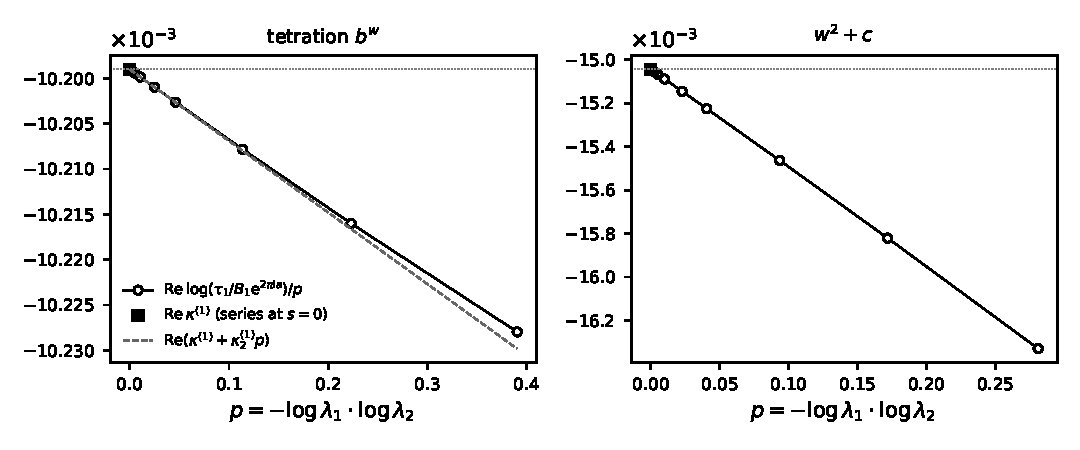
\includegraphics[width=\textwidth]{figures/fig8_deficit.pdf}
\caption{$\Rea\log(\tau_1/B_1\ee^{2\pi\ii a})/p$ 随 $p$ 的变化（圆圈，双曲侧直接计算，$\lambda_1=0.5,\dots,0.98$），
方块为 $s=0$ 处级数给出的 $\Rea\kappa^{(1)}$。左：tetration，虚线为 $\Rea(\kappa^{(1)}+\kappa^{(1)}_2p)$；右：二次族 $w^2+c$。数值。}
\label{ch8:fig:deficit}
\end{figure}

% ======================================================================
\notes

\paragraph{来源.}
本章是 \cite{KneserPaper} §5（The first-order term: a parabolic series）对一般实鞍结开折的改写。对应关系：
\cref{lem:uniform-model}–引理~5.1（对角元 $i/2$ 换成 $ia_2$，$D=8s$ 换成 $4\gamma s/a_2$）；\cref{ch8:lem:finite}–引理~5.2（$-2/u$ 换成 $-1/(a_2u)$）；
\cref{ch8:lem:derbounds}–引理~5.3；\cref{ch8:prop:diff}–命题~5.4；\cref{thm:first-order}–定理~5.6（$p'(0)=2$ 换成 $4a_2\gamma$）；
\cref{ch8:prop:higher}–命题~5.7；\cref{thm:all-orders}–定理~5.8（编号均指论文）。一般化的清单见论文定理~9.4 与 \texttt{docs/general-statements-zh.md} §2.6。
与论文相比，这里补了两处：\cref{lem:uniform-model}(3)（$e_i(0)=d_i$，论文只在注中说明）与除法公式 \eqref{ch8:eq:division}；
排斥侧的反射逆在一般情形下没有显式公式，只用到它对 $(s,v)$ 联合全纯。

\paragraph{思路.}
一致模型的想法来自 Mardešić--Roussarie--Rousseau 的预备形式 \cite{MRR2004}：在开折的整个参数邻域上同时正规化两个不动点。
发现``逐项求导发散''以及用一致模型修正的过程记录在 \texttt{docs/mrr-first-order-zh.md}。注意 \eqref{ch8:eq:Adot} 不同于朴素的 Hadamard 有限部分正则化：
后者的常数项一般不等于真导数，一致模型把正则化变成了精确恒等式。

\paragraph{变分公式.}
\cref{thm:first-order} 把 $\kappa^{(n)}$ 表示为一个收敛级数，但没有说明它的含义。第~\ref{ch:variation} 章证明
$\kappa^{(n)}=\kappa^{(n)}_{\mathrm{tr}}(g)+\Dfun_n(g)[X-X(0)]/(4a_2X(0))$：法向部分是芽的平移开折的一阶项，切向部分是 horn 不变量沿抛物层的导数。
那里的证明把本章的一致模型放进 Banach 空间 $\Ocal_r$ 中，作为 $f$ 的全纯函数。

% ======================================================================
\exercises

\begin{exercise}\label{ch8:ex:udot}
设 $u_k=g^k(u)$，$u\in P_R$。证明 $u_k=-\frac1{a_2k}+O(k^{-2}\log k)$，并由 $\dot u_{k+1}=g'(u_k)\dot u_k-X(u_k)$ 证明 $\dot u_k=-\frac{\gamma}3k+O(\log^2k)$。
\end{exercise}
\begin{hint}
令 $\dot u_k=k\,y_k$，得到 $y_{k+1}=y_k-\frac3k\bigl(y_k+\frac\gamma3\bigr)+O(k^{-2}\log k)$。
\end{hint}

\begin{exercise}\label{ch8:ex:divergence}
对第~\ref{ch:confluence} 章的（未修正的）模型时间，利用习题~\ref{ch8:ex:udot} 证明 $\partial_s[F_s(u_k)]_{s=0}+F_0'(u_k)\dot u_k\to-\frac{\gamma}{3a_2}\varphi_0(0)$，
其中 $F_0(u)=\varphi_0(0)u^2+O(u^3)$。对 tetration 求出 $\varphi_0(0)$，确认它不为零。
\end{exercise}

\begin{exercise}\label{ch8:ex:hadamard}
设 $G$ 在凸区域上全纯。证明 $(x,y)\mapsto(G(x)-G(y))/(x-y)$（对角线上取 $G'(x)$）联合全纯。由此补全 \cref{ch8:lem:removable} 中``被 $x-y$ 整除''一步。
\end{exercise}

\begin{exercise}\label{ch8:ex:p-holo}
用 \cref{ch8:lem:removable} 的论证（偶函数 $\Rightarrow$ $t^2$ 的函数）直接证明 $p=-\log\lambda_1\log\lambda_2$ 是 $s$ 的全纯函数，并对 tetration 验证 $p=2s+\frac{10}9s^2+O(s^3)$。
\end{exercise}

\begin{exercise}\label{ch8:ex:N2}
对 $g(u)=u+u^2$ 取 $N=3$。写出 \cref{lem:uniform-model} 证明中的 $4\times4$ 下三角矩阵 $M(0)$ 与 $\mathrm{rem}(\Phi_0)$，解出 $e(0)$，
并验证它给出形式 Abel 函数的系数 $d_1=-\frac12$、$d_2=\frac13$、$d_3=-\frac{13}{36}$、$d_4=\frac{113}{240}$（与 \cref{ch8:exa:quad-model} 的 $N=2$ 结果相容）。
\end{exercise}

\begin{exercise}\label{ch8:ex:exponent}
在 \cref{ch8:prop:diff} 的平衡中取 $J=s^{-\beta}$，求使误差最小的 $\beta$，证明误差为 $O(s^{2-8/(2N+3)})$。$N=2$ 时得到什么？
\end{exercise}

\begin{exercise}\label{ch8:ex:base}
由 \cref{prop:base-point} 证明：换基点使 $\kappa^{(n)}$ 改变 $\frac{2\pi\ii n}{4a_2\gamma}\Delta'(0)$，其中 $\Delta(s)=R_s^{-1}(w_0')$ 关于 $s$ 的导数在 $0^+$ 处存在。
所以 $\Rea\kappa^{(n)}$ 与基点无关。
\end{exercise}

\begin{exercise}\label{ch8:ex:CR}
设 $L_1=|\log\lambda_1|$、$L_2=\log\lambda_2$，$\epsilon_{\mathrm{CR}}=(A_2-A_1)^{-2}$，$\nu=A_1+A_2$。验证 $p=L_1L_2=4\epsilon_{\mathrm{CR}}/(1-\nu^2\epsilon_{\mathrm{CR}})$。
\end{exercise}

\begin{exercise}\label{ch8:ex:beyond}
设 $\phi(s)$ 在 $(0,s_0]$ 上有渐近展开 $\sum_ja_js^j$。证明 $\phi(s)+O(\Lam)$ 有同一个展开。由此说明 \cref{ch8:cor:sewing} 中 $\hat c_n$ 与 $\tau_n$ 的差别在任何阶的渐近展开中都看不见，
只能从指数小的尺度上看到。
\end{exercise}

\begin{exercise}\label{ch8:ex:fit}
用第~\ref{ch:confluence} 章数值一节的表中二次族的 $|\tau_1|/|B_1|-1$，通过对 $p$ 的二次拟合估计 $\Rea\kappa^{(1)}$，与级数值 $-0.0150441028391897$ 比较。
解释为什么 $(|\tau_1|/|B_1|-1)/p$ 与 $\Rea\log(\tau_1/B_1\ee^{2\pi\ii a})/p$ 只在 $O(p)$ 上不同。
\end{exercise}

\begin{exercise}\label{ch8:ex:second}
（较难）写出 $\kappa^{(n)}_2$ 用 $\cfA^{(1)},\cfA^{(2)},\cfS^{\sharp(1)},\cfS^{\sharp(2)}$ 及其导数在 $\ell$ 上的 Fourier 系数表示的公式。
\end{exercise}
\begin{hint}
先把 $v_s$ 展开到 $s^2$：$v_s=v+sV_1+s^2V_2+O(s^{2+\vartheta})$，$V_1=-\cfS^{\sharp(1)}/\Phirep'$，$V_2$ 由 $\cfS^\sharp_s(v_s)=z$ 的 $s^2$ 项确定；再展开 $\cfA_s(v_s)$，最后把 $s$ 换成 $p$。
\end{hint}
